\vspace{-6pt}

\section{Design and Implementation}
\label{sec:design}
Our experiments so far have demonstrated that the length of the prefix shared across \textit{all} active requests is an important determinant of system performance. However, this metric interacts with batch size in a complex way: larger batches improve GPU utilization but often reduce shared prefix alignment. Further, detecting this shared prefix length incurs high overhead in existing systems. We now describe the design of \Feather, an efficient scheduler that finds the right balance between batch size and prefix homogeneity. 

\vspace{-7pt}

\subsection{Overview}
\label{sec:system_overview}
\Feather is based on the following two key ideas.

\vspace{-6pt}

\subsubsection*{Key Idea 1: Learn the Stopping Decision via RL (\S\ref{subsec:batching_rl})}
The trade-off between batch size and prefix homogeneity raises a key question: when should the scheduler stop adding requests? The answer depends on both hardware and workload, making fixed heuristics brittle. We model batch construction as a sequential decision process and learn a stopping policy via Reinforcement Learning. At each step, the scheduler evaluates a candidate request using various state features and decides whether it should be added to the batch or if the batch should be dispatched to the GPU for execution.

\vspace{-6pt}

\subsubsection*{Key Idea 2: Shared Prefix Detection via Chunked Hash Tree (\S\ref{subsec:chunked_hash_tree})}
Tree-based approaches incur significant overhead (\S\ref{subsec:overhead_dynamic_prefix_detection}), and finding the best waiting request requires a DFS traversal that is $\mathcal{O}(E)$, where $E$ is the number of edges in the radix tree. In the worst case, this can go up to $\mathcal{O}(W\times T)$, where $W$ is the number of waiting requests, and $T$ is the sequence length. We instead represent each request as a sequence of hashes over fixed-size chunks and maintain a working set of hashes for the active batch. This is similar in spirit to Merkle-style hash chains, but it does not require sequential hash computation, and each chunk can be processed independently without prefix dependencies. Prefix matching is thus reduced to a set-overlap problem: selecting the request with the maximum overlap with the working set. However, a naive implementation that scans all requests and counts overlaps requires $\mathcal{O}(W \cdot C)$ work per decision, where $C$ is the number of chunks in a request, which remains too expensive for frequent scheduling. We avoid this by maintaining a missing count per request—the number of chunks absent from the working set—which changes only when the working set changes (i.e., upon request addition or completion). Overlaps are thus updated incrementally, reducing selection to finding the request with the smallest missing count. To do so efficiently, we maintain a min-heap over missing counts, pushing updates and using lazy deletion to discard stale entries, yielding $\mathcal{O}(\log W)$ selection cost.

\vspace{-5pt}

\subsubsection*{System Architecture}
Figure~\ref{fig:pipeline} shows the overall scheduling pipeline. We consider an inference server that continuously receives requests, which are inserted into the waiting queue of CHT. The scheduler builds batches incrementally in a loop. It first finds the best candidate by retrieving the waiting request with the highest overlap with the current working set. Then the RL policy evaluates the current system state and decides whether to \textsc{Add} the request or \textsc{Stop}. If \textsc{Add} is chosen, the request is added to the scheduler batch, and all the data structures, such as the working set and the min-heap, are updated accordingly; otherwise, the batch is dispatched to the GPU for an execution step. The decode throughput measured after the GPU execution is used as a reward for the RL policy. Completed requests are removed from the active batch, and the working set is updated.

\begin{figure}[t]
\centering
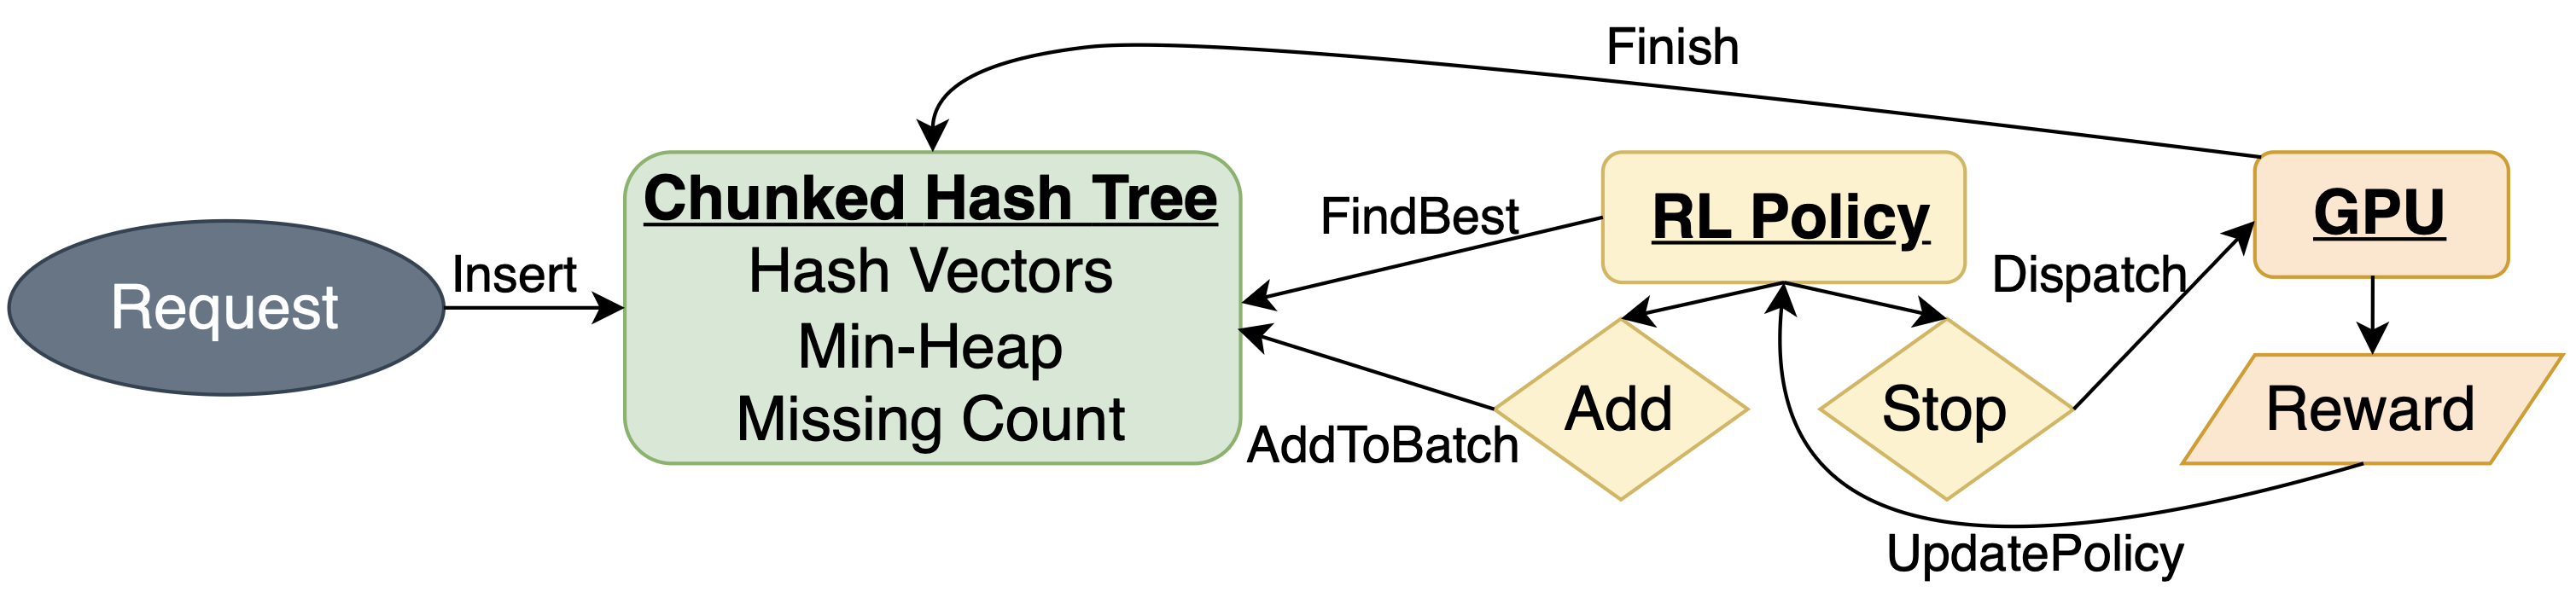
\includegraphics[width=\columnwidth]{illustration_images/pipeline.png}
\caption{\Feather Pipeline}
\label{fig:pipeline}
\vspace{-15pt}
\end{figure}

\vspace{-7pt}

\begin{figure*}[t]
\captionsetup[subfigure]{labelformat=simple}
    \renewcommand\thesubfigure{(\alph{subfigure})}
\centering
\begin{subfigure}{0.24\textwidth}
    \centering
    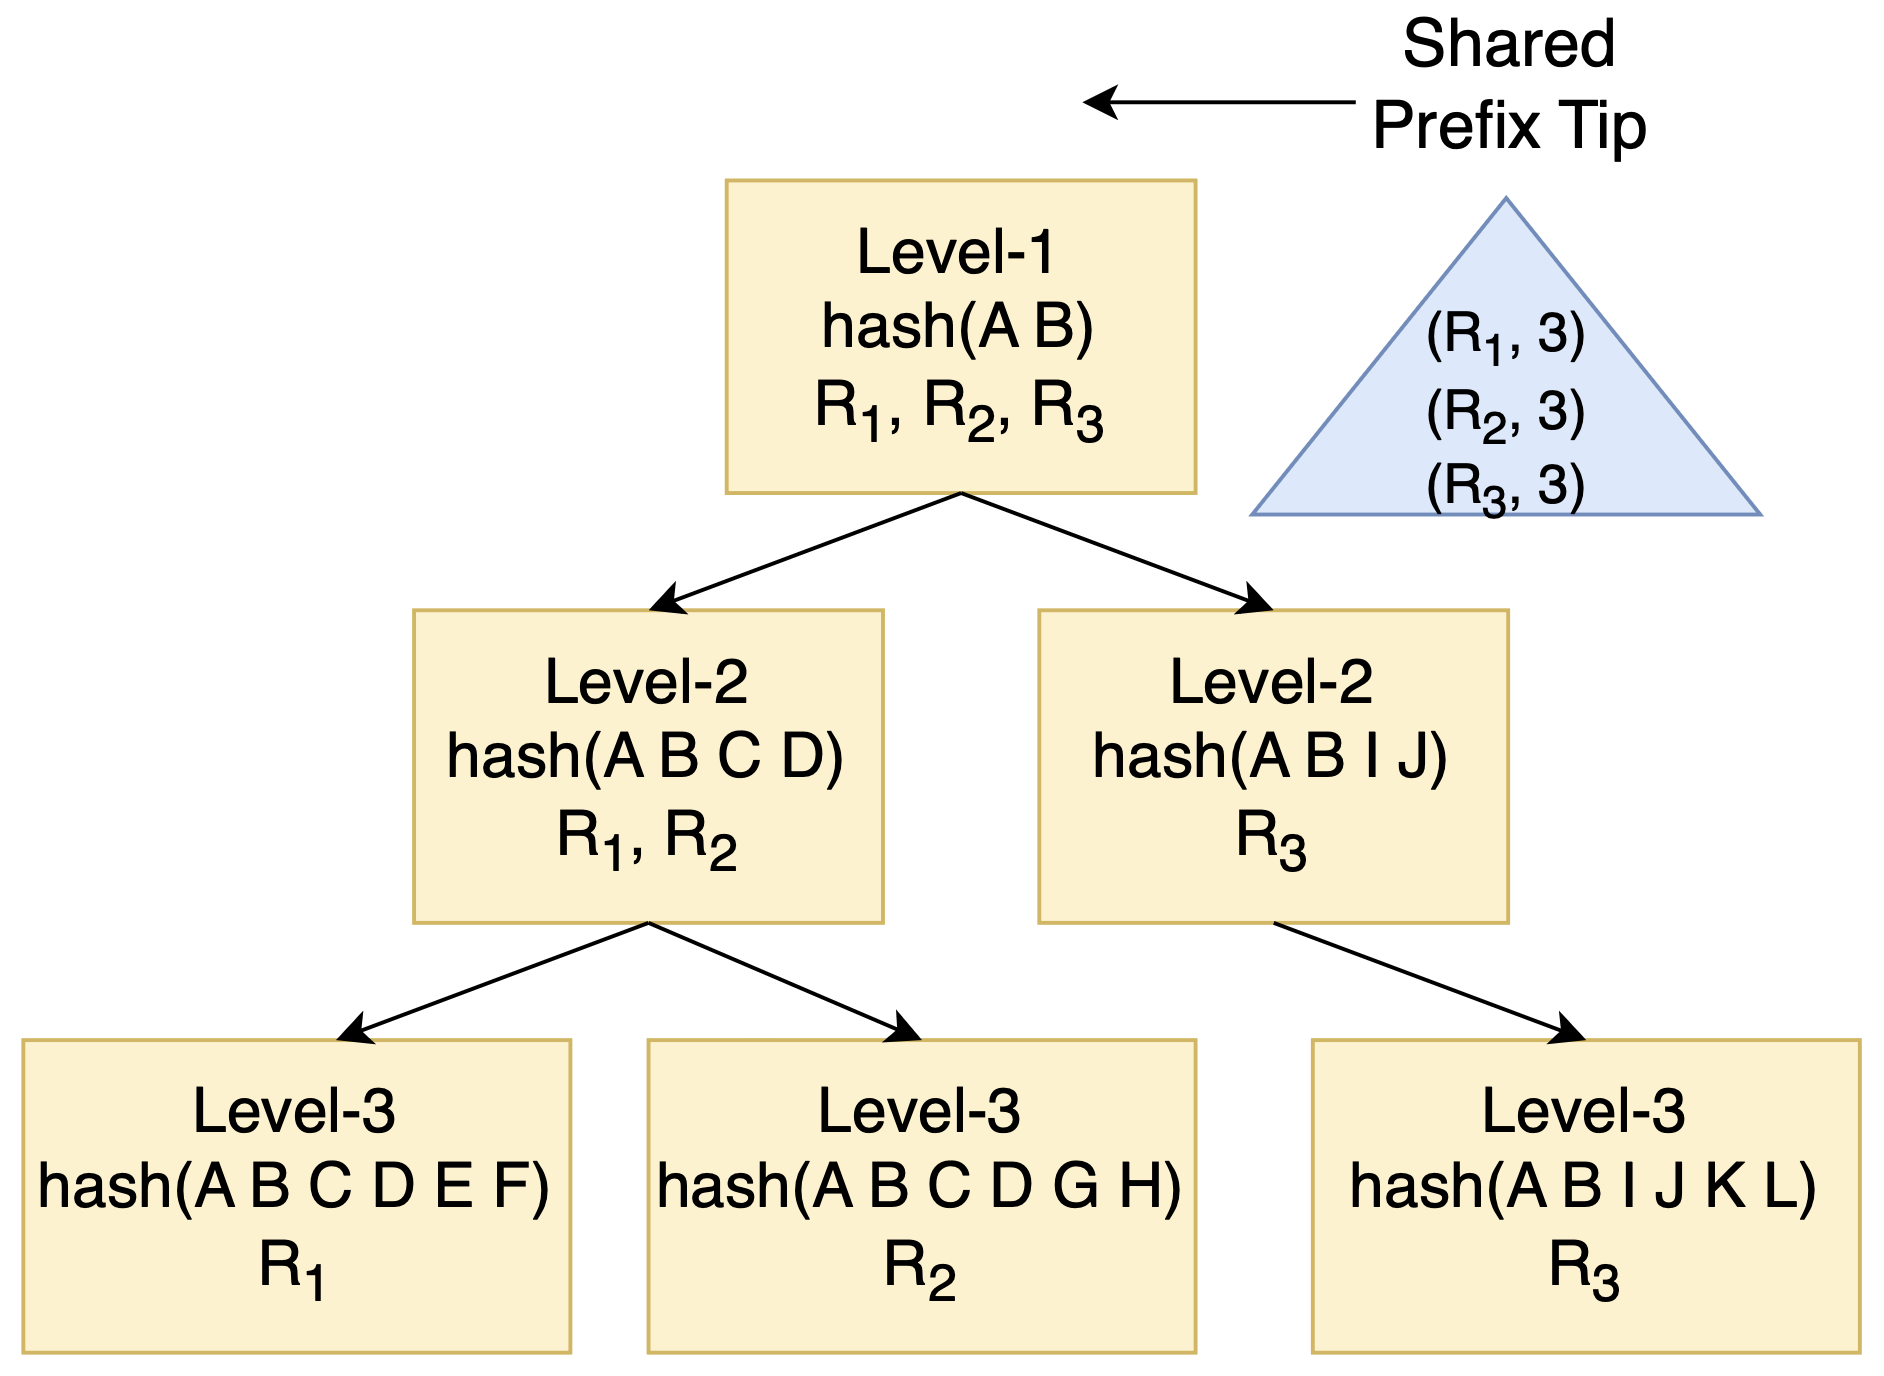
\includegraphics[width=\linewidth]{illustration_images/chunked_hash_tree_insertion.png}
    \caption{Insertion}
    \label{fig:chunked_hash_tree_insertion}
\end{subfigure}
\hfill
\begin{subfigure}{0.28\textwidth}
    \centering
    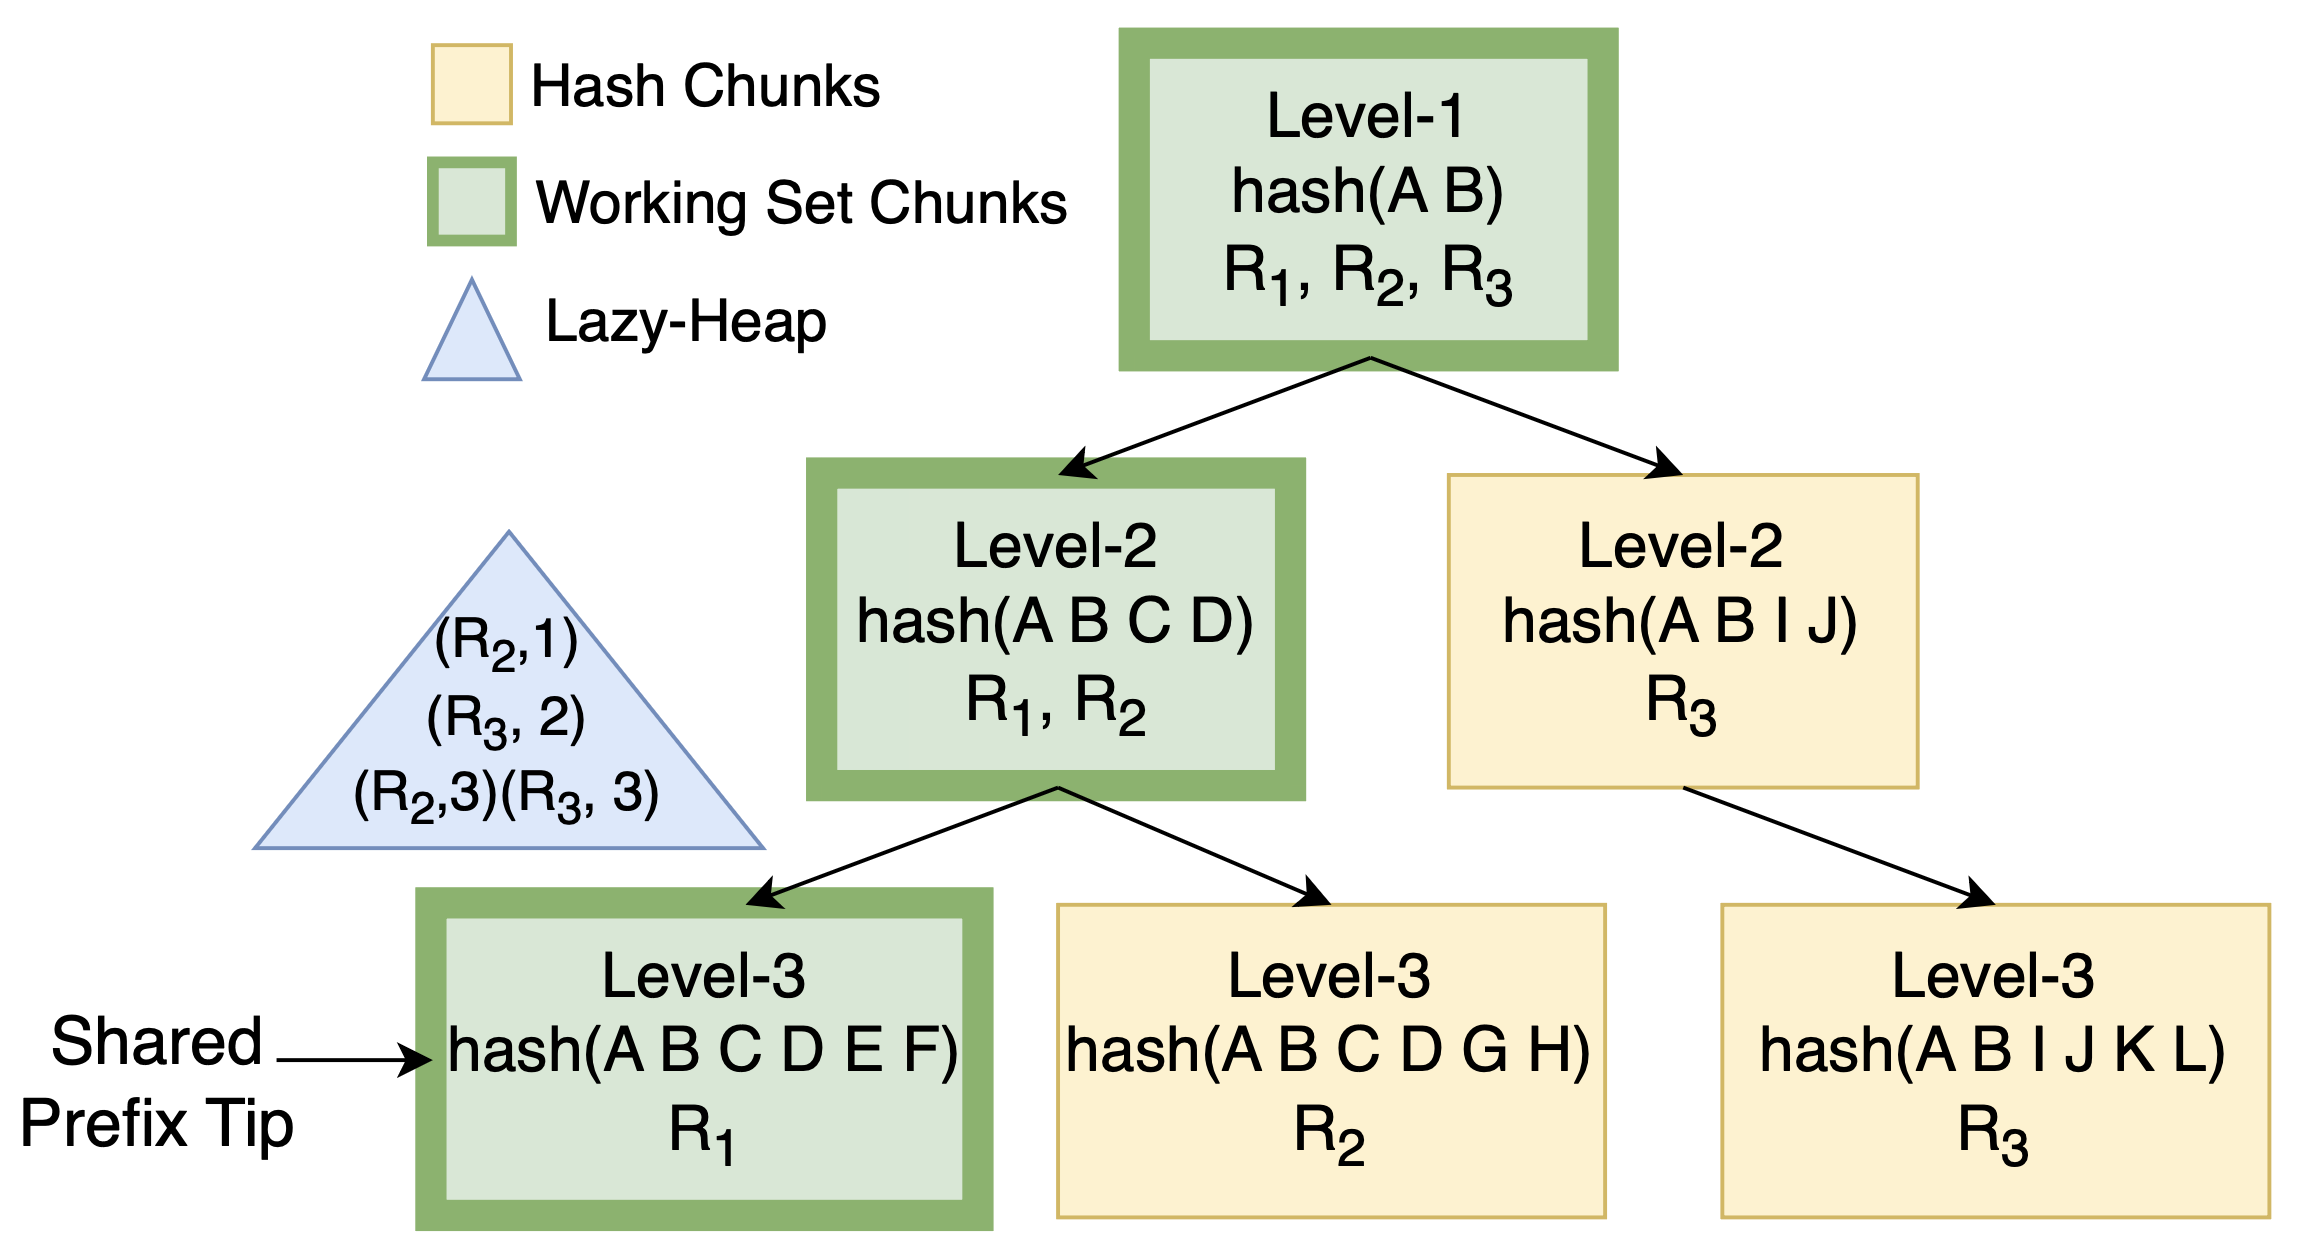
\includegraphics[width=\linewidth]{illustration_images/chunked_hash_tree_activation.png}
    \caption{Adding to Batch}
    \label{fig:chunked_hash_tree_activation}
\end{subfigure}
\hfill
\begin{subfigure}{0.24\textwidth}
    \centering
    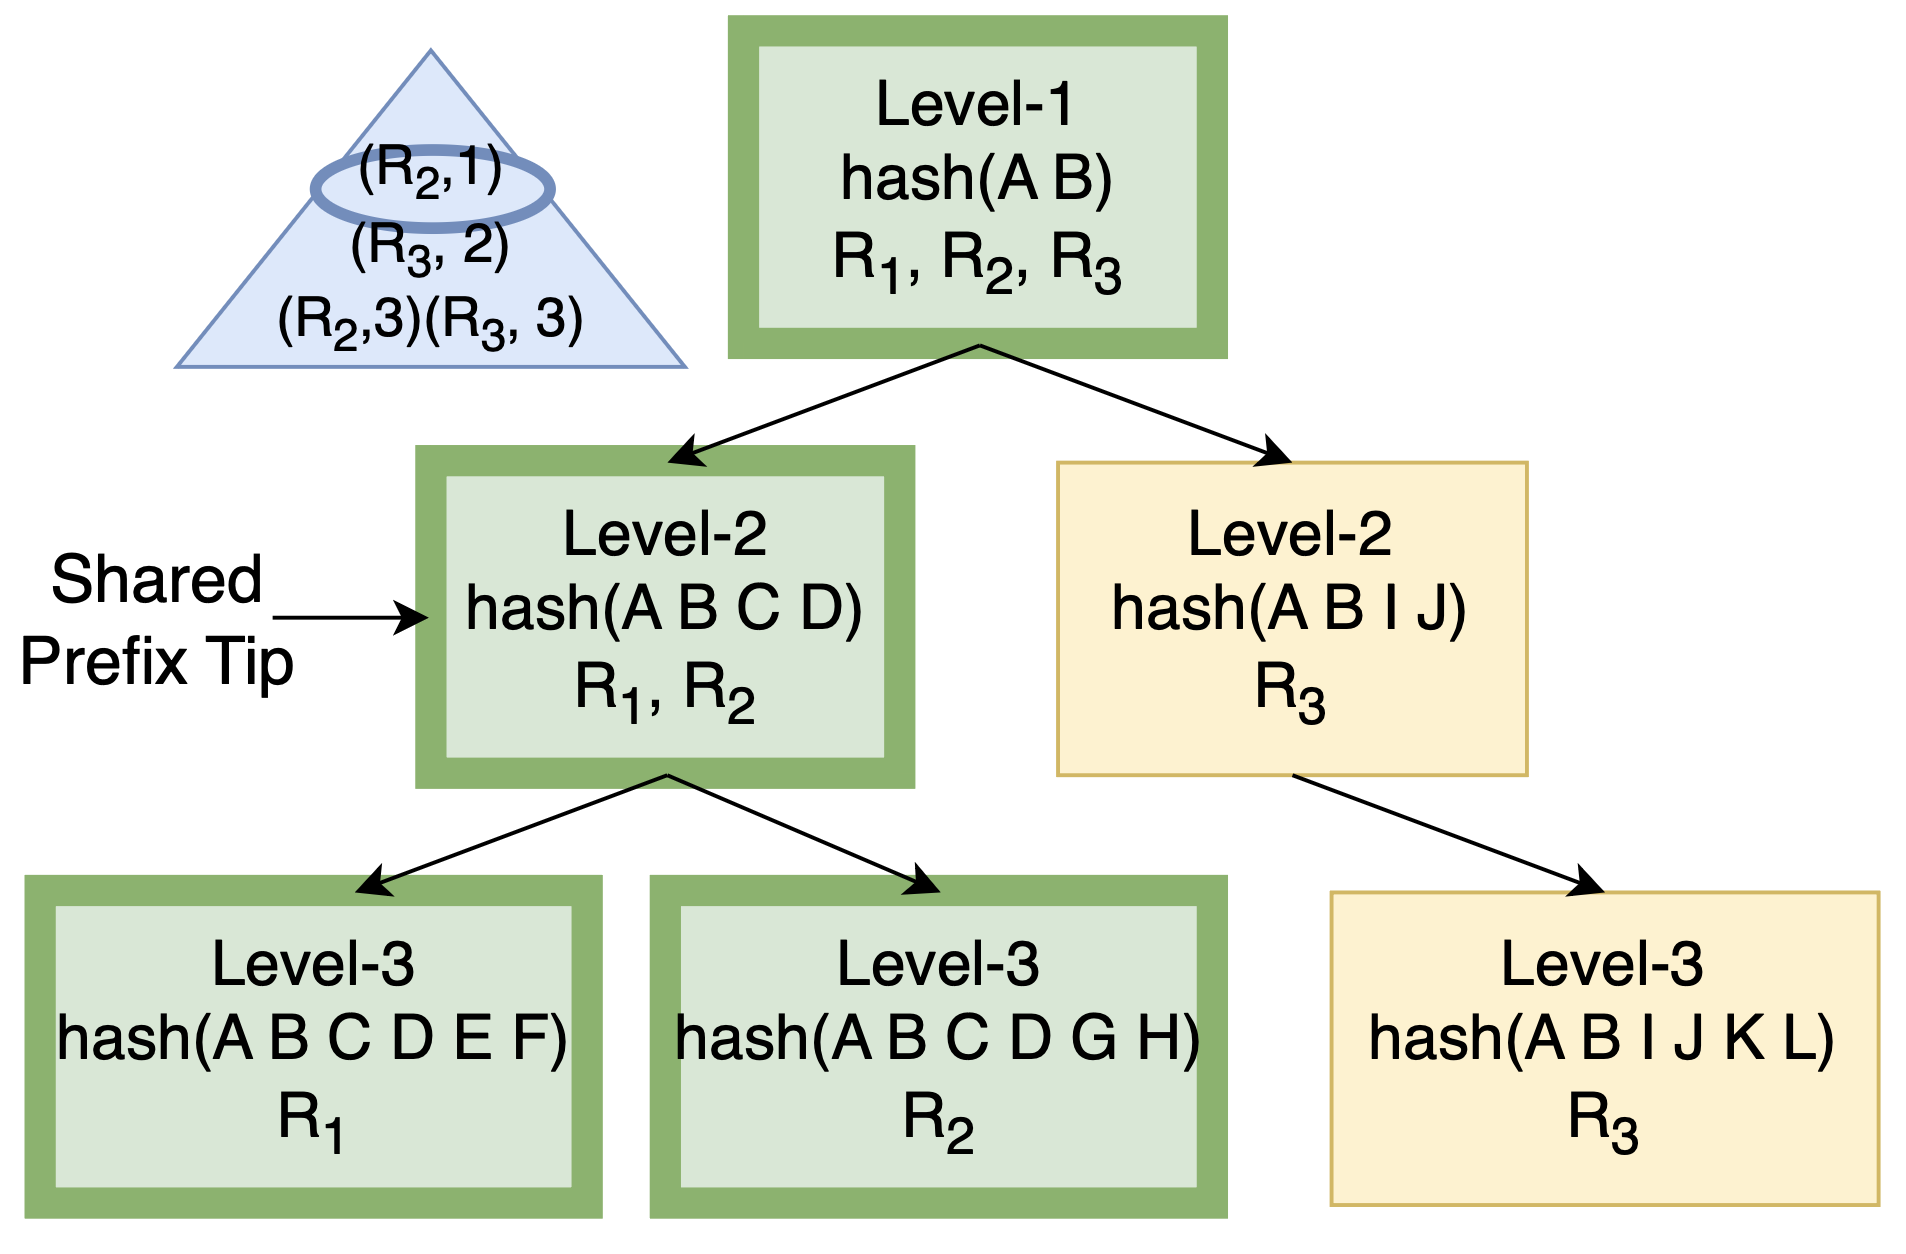
\includegraphics[width=\linewidth]{illustration_images/chunked_hash_tree_find_best_request.png}
    \caption{Finding the Best Request}
    \label{fig:chunked_hash_tree_find_best_request}
\end{subfigure}
\hfill
\begin{subfigure}{0.21\textwidth}
    \centering
    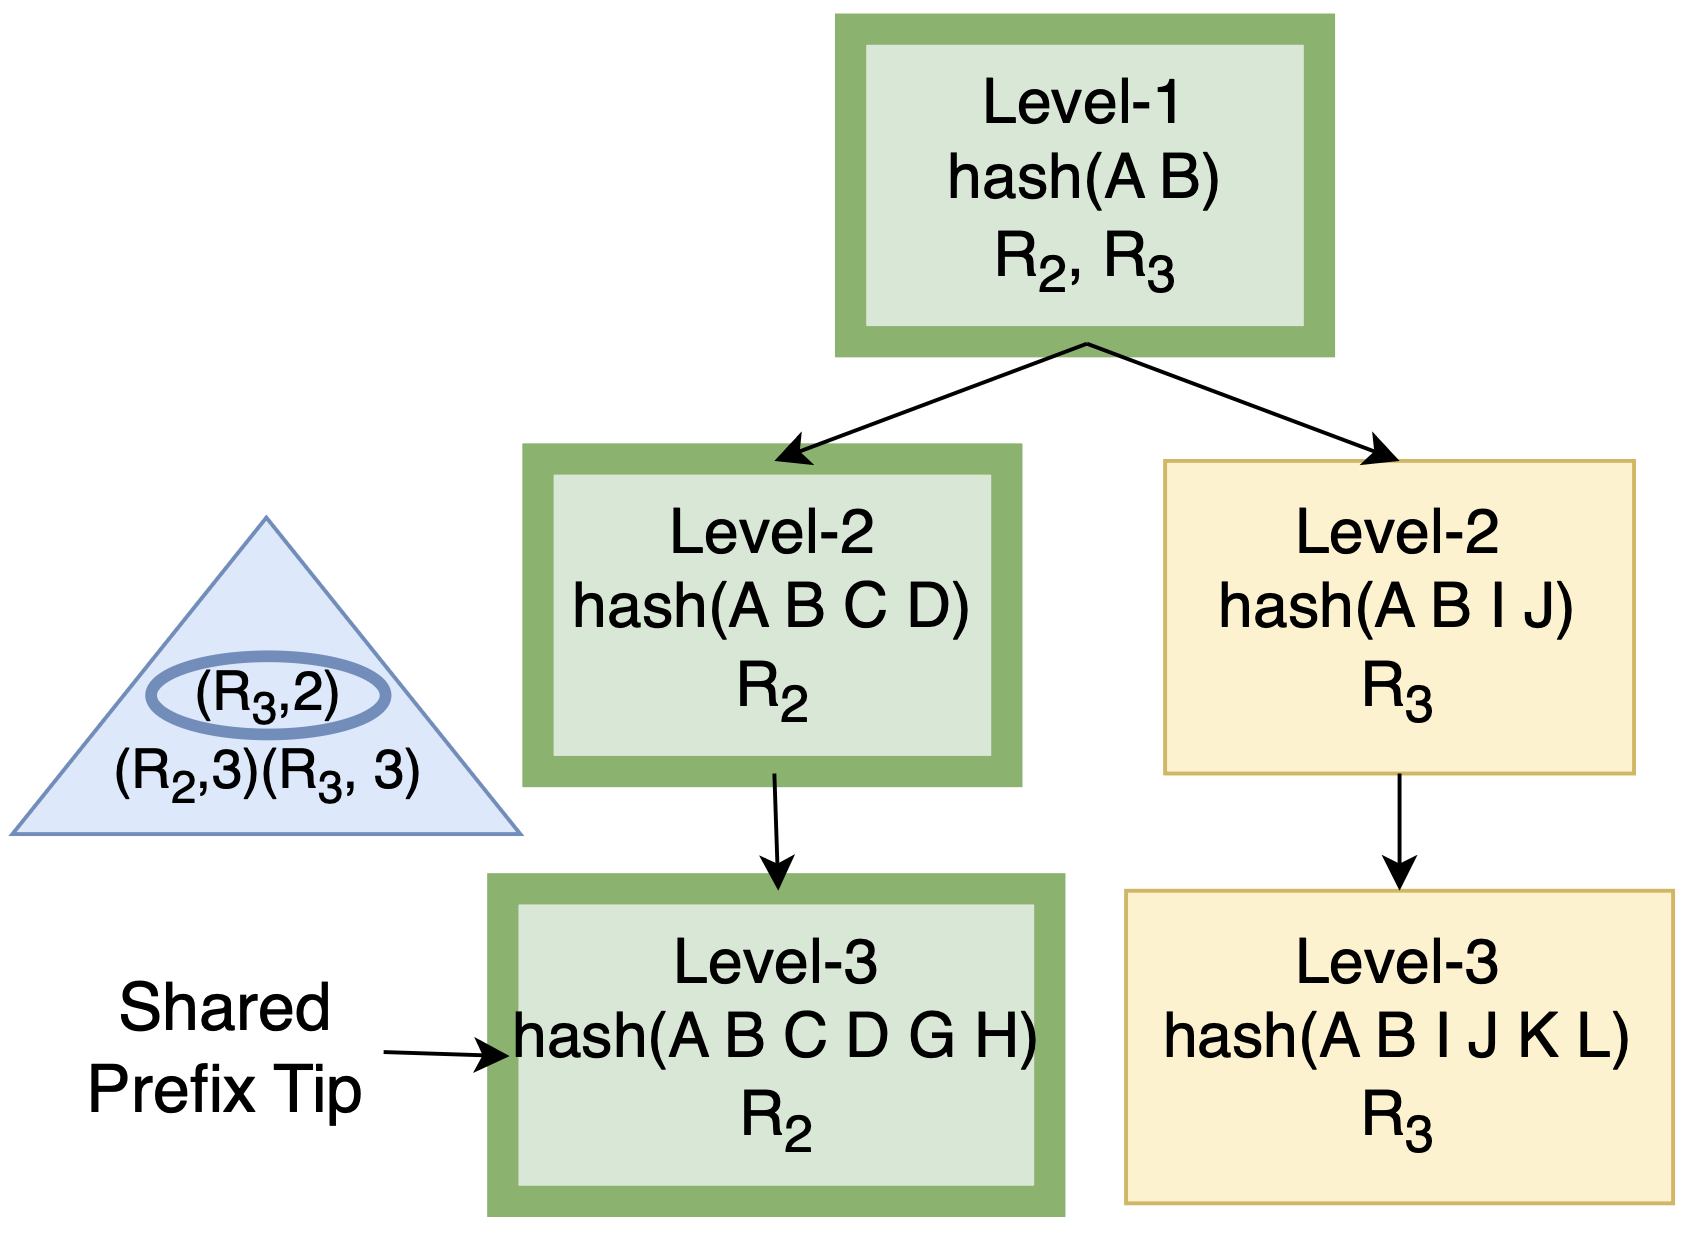
\includegraphics[width=\linewidth]{illustration_images/chunked_hash_tree_finish.png}
    \caption{Request Completion}
    \label{fig:chunked_hash_tree_finish}
\end{subfigure}
\caption{Chunked Hash Tree Operations}
\label{fig:chunked_hash_tree}
\vspace{-15pt}
\end{figure*}

\subsection{Chunked Hash Tree (CHT)}
\label{subsec:chunked_hash_tree}
We now describe the operations of CHT (a more formal treatment is in \S\ref{sec:algorithms}). We begin with how token sequences are mapped to a compact representation in our system.

\vspace{-5pt}

\subsubsection*{Hash Vectors}
Given a request as a token sequence, we partition it into non-overlapping chunks of size $K$ and build a sequence of hashes, one for each chunk, where each hash is cumulative over all tokens up to that chunk. For example, in Figure~\ref{fig:chunked_hash_tree_insertion}, a request with tokens A-F and $K = 2$ is represented as three incremental hashes: hash(A-B), hash(A-D), and hash(A-F). Two requests will have the same hash at level $l$ iff they share the same first $lK$ tokens. Each request is represented as an ordered hash vector. We use an incremental xxHash-64 state, ensuring each token is processed once, yielding a total cost of $\mathcal{O}(T)$, independent of the number of chunk boundaries, where $T$ is the sequence length.



\vspace{-5pt}

\subsubsection*{Insertion}
\textsc{Insert} is invoked when a new request arrives at the scheduler. We first compute the cumulative prefix-hash vector and store it in a map from request IDs to hash vectors for faster reuse. We also maintain a reverse index that maps each hash to the set of requests containing that hash. For each hash in the hash vector, we insert the request into this reverse index. The overall cost is dominated by the hash computation phase, which runs in $\mathcal{O}(T)$.

\vspace{-5pt}

\subsubsection*{Working Set, Min-Heap and Shared Prefix Tip}
To evaluate how well a request matches the active batch, we maintain a working set that contains (level, hash) tuples representing prefix hashes at that level covered by currently active requests. For each request, we also maintain a missing count, which is the number of levels for which this request's hashes are not present in the working set. We insert these missing counts into a min-heap, which enables efficient retrieval of the most suitable request for addition to the batch. \textsc{Insert} updates both of these structures. Moreover, we do not perform in-place updates and use lazy deletion to discard stale entries in the heap. To relate to our key metric, which is the number of chunks shared by all active requests, we also maintain a shared prefix tip, storing the depth and hash of the deepest node that is shared by all the active requests. Figure~\ref{fig:chunked_hash_tree_activation} shows the Chunked Hash Tree after the request $R_1$ is added to the batch. The nodes marked in green denote the working set. Since there is just a single request, the shared prefix tip is at Level-3 of $R_1$. The heap contains the missing counts of the waiting requests along with stale entries. 

\vspace{-5pt}

\subsubsection*{Finding the Best Request}
The goal of \textsc{FindBest} is to select the waiting request that best complements the active batch, i.e., the one with the minimum missing count, so that we maximize the depth of the shared prefix tip\footnote{An astute reader might ask why we are choosing a request based on its difference from the working set rather than its impact on the length of the shared prefix tip. A brief explanation is that we want to pick a request that helps us revert back to a longer shared prefix tip sooner, and a request that differs from the working set by the least number of chunks helps us achieve this goal best. We refer the reader to Appendix~\ref{subsec:find_best_reques_alternative_heuristic} for more details.}. Since the min-heap is keyed by this count, the best candidate appears at the top after skipping stale entries. As shown in Figure~\ref{fig:chunked_hash_tree_find_best_request}, $R_2$ appears at the top of the min-heap and is therefore selected as the best request. Note that adding $R_2$ to the batch reduces the shared prefix tip by one level. \textsc{FindBest} runs in $\mathcal{O}(\log W)$, where $W$ is the number of waiting requests. For the selected request, we compute two metrics that are inputs to the RL policy (\S\ref{subsec:batching_rl}), which needs to decide whether adding the request to the current batch is beneficial for the overall throughput. One of the metrics is the change in the depth of the shared prefix tip, and the other is the number of additional waiting requests that are present at this new depth, which can all be added to the batch without any further impact on the shared prefix tip in the future. 

\vspace{-5pt}

\subsubsection*{Adding a Request to the Active Batch} 
When a request is promoted to the active batch, we update the working set to include its prefixes and recompute the shared prefix tip. We iterate over the hash vector backwards; for each level, if the corresponding prefix hash isn't present in the working set, it is inserted, and all waiting requests sharing it have their missing count decremented. For the shared prefix tip, admitting a new request can only \textit{shorten} the common prefix, so we seek the deepest level where it agrees with the existing tip hash. This corresponds to the least common ancestor of all active request leaves in the hash trie. \textsc{AddToBatch} runs in $\mathcal{O}(C \cdot W_h \cdot \log W)$ time, where $C = \lceil T/K \rceil$ is the number of chunks for a request with $T$ tokens, and $W_h$ is the number of waiting requests that share the same hash ($W_h \ll W$).

\vspace{-5pt}

\subsubsection*{Removing a Request from the Active Batch}
\textsc{Finish} is called when a request completes, and we remove it from the active batch. It is the symmetric counterpart of \textsc{AddToBatch}. We iterate over the hash vector from the start. A hash unused by any active request is removed from the working set, and all waiting requests containing it have their missing count incremented. A request completion can only \textit{lengthen} the shared prefix tip since the remaining active requests may agree on a longer common prefix. Starting from the tip's previous position, we scan forward, checking whether all remaining active requests share the same hash at each level. (We do this efficiently by maintaining reference counts of each hash.) The extension stops at the first level of disagreement or at the shortest active request. This scan is inexpensive in practice, as the tip rarely advances more than a few levels. \textsc{Finish} also runs in $\mathcal{O}(C \cdot W_h \cdot \log W)$ time. Figure~\ref{fig:chunked_hash_tree_finish} shows the state after $R_1$ completes: the tip extends to $R_2$'s final level, and waiting heap costs are updated accordingly. 

\vspace{-5pt}

\subsubsection*{Optimizations}
We employ several optimizations to improve efficiency. First, \textsc{FindBest} may be invoked multiple times within a scheduling round without state changes, so we cache its last result and reuse it until it is invalidated by any mutation (e.g., \textsc{AddToBatch} and \textsc{Finish}). Second, we use lazy heap updates: when a request's missing count changes, we push a new entry instead of updating it in place and skip stale entries during \textsc{FindBest}. Third, we maintain the shared prefix tip incrementally rather than recomputing it. This drops the cost from $\mathcal{O}(A \cdot C)$, where $A$ is the number of active requests, and $C$ is the number of chunks, to just $\mathcal{O}(C)$ in the worst case and typically terminates earlier. Finally, all major data structures are pre-allocated at initialization to eliminate rehashing and reallocation overhead. 

\vspace{-7pt}

\subsection{Batching and Reinforcement Learning}
\label{subsec:batching_rl}
The CHT efficiently identifies the next best request to add, maximizing shared prefix length, but it does not determine \textit{when to stop}. While adding requests improves GPU utilization, it can also shrink the shared prefix and degrade locality. We frame this stop/continue decision as a learning problem and present three policies: a heuristic, a contextual bandit, and a Q-learning agent. The scheduler incrementally builds a batch by selecting candidates via the CHT and deciding whether to admit them or dispatch the batch.

\vspace{-6pt}

\subsubsection*{State, Actions, and Reward}
At each step of batch formation, the scheduler observes the state $s = (\mathit{b},\; \Delta,\; \mathit{w})$ and takes an action $a \in \{\textsc{Add}, \textsc{Stop}\}$. Here, $b$ is the current batch size (a proxy for GPU utilization), $\Delta$ is the loss in the shared prefix, and $w$ is the number of waiting requests sharing the prefix up to the new depth, indicating whether the locality cost of this addition will be compensated by future activations. Both RL policies optimize the reward $\mathcal{R} = \text{throughput}_{\mathrm{decode}}$. Maximizing this encourages large batches and short decode times (better prefix locality). The state is discretized into $(\hat{b}, \hat{\Delta}, \hat{w})$, where $b$ and $w$ use exponential bins, and $\Delta$ uses coarse thresholds. The resulting table is small, hashable, and converges quickly under moderate load.

\vspace{-6pt}

\subsubsection*{Heuristic Policy}
As a baseline, we encode domain intuition as simple rules balancing two goals: maximizing GPU utilization (large batches) and preserving prefix locality (avoiding large drops in the shared chain). The heuristic always accepts candidates with zero chunk loss (free additions). When the batch is small, it tolerates higher loss to avoid underutilization. Otherwise, it admits a candidate only if the chunk loss is within a fixed threshold, with slightly relaxed tolerance when many waiting requests share the resulting prefix (anticipating amortization). If none of these conditions hold, it stops and dispatches the batch. This policy requires no training and converges immediately, but its fixed thresholds cannot adapt to workload or hardware changes.

\vspace{-6pt}

\subsubsection*{Contextual Bandit}
To avoid hand-tuned thresholds, we use a contextual bandit with Upper Confidence Bound (UCB) selection~\cite{auer2002finite}. Each batch-construction step is treated as an independent decision: given the discretized state $\hat{s} = (\hat{b}, \hat{\Delta}, \hat{w})$, the policy selects the action that maximizes

\vspace{-10pt}

\[
  \mathrm{UCB}(\hat{s},a) = \frac{\mu(\hat{s},a)}{n(\hat{s},a)} + c\sqrt{\frac{\ln S}{n(\hat{s},a)}}.
\]

\vspace{-6pt}

Here, $\mu(\hat{s}, a)$ is the cumulative reward, $n(\hat{s}, a)$ is the number of times action $a$ was taken in $\hat{s}$, $S$ is the total number of decisions, and $c$ is the exploration coefficient. The first term favors high-reward actions, while the second promotes exploration of under-sampled ones. 

\vspace{-5pt}

\subsubsection*{Q-Learning Policy}
As an alternative to the previous policy, we can also model batch construction as an episodic reinforcement learning problem, where each episode begins when forming a new batch and ends upon \textsc{Stop} or when the waiting queue is exhausted. The Q-table~\cite{watkins1992} stores values $Q(s, a)$ for each (discretized state, action) pair and is updated after each episode using:

\vspace{-14pt}

\[
Q(s, a) \; \leftarrow\; Q(s, a) + \alpha\bigl[r + \gamma \max_{a'} Q(s', a') - Q(s, a)\bigr].
\]

\vspace{-6pt}

Here, $r$ is the observed throughput, $s'$ is the next state, $\alpha$ the learning rate, and $\gamma$ the discount factor, which biases the agent toward near-term throughput, consistent with real-time inference. We follow an $\varepsilon$-greedy exploration strategy: at each step, a random action is selected with probability $\varepsilon$, and the greedy action $\arg\max_a Q(s,a)$ otherwise. During training, $\varepsilon$ decays from $1.0$ to $\varepsilon_{\min}$, transitioning from full exploration to near-deterministic behavior. Qualitatively, we expect this policy to perform better in the long term when actions influence future batch composition.

At each step, \textsc{FindBest} returns the lowest-cost candidate along with $(\Delta, w)$, forming the state $s$. The policy (heuristic, bandit, or Q-learning) then selects \textsc{Add} or \textsc{Stop}. If \textsc{Add}, the request is activated and appended to the batch; otherwise, the batch is dispatched. After execution, the observed decode throughput is used as the reward: the bandit updates its statistics and the Q-learning agent applies the Bellman update. This has also been shown in Figure~\ref{fig:pipeline}. 

\vspace{-7pt}

\subsection{Integration with vLLM and SGLang}
We integrate our scheduler as a lightweight layer on top of both vLLM~\cite{kwon2023efficient} and SGLang~\cite{zheng2024sglangefficientexecutionstructured}. The Chunked Hash Tree (implemented in C++) along with shared prefix chain tracking and reinforcement learning policies operates entirely at the scheduler level. We will upstream our changes to these repositories upon acceptance of our publication.

\vspace{-3pt}